% Manuscript formatted for International Ophthalmology.
% Springer Nature LaTeX template, Original Article.
\documentclass[pdflatex,sn-vancouver,Numbered,iicol]{sn-jnl}

\usepackage{graphicx}
\usepackage{xcolor}
\usepackage{booktabs}
\usepackage{amsmath,amssymb}
\usepackage{manyfoot}
\usepackage{url}

\begin{document}

\title[Source and label effects in ROP AI benchmarks]{Dataset source and label
reference alter performance estimates in public retinopathy of prematurity AI
benchmarks}

\author[1]{\fnm{Jin} \sur{Luo}}

\author[2]{\fnm{Dongwei} \sur{Guo}}

\author[3]{\fnm{Xinsi} \sur{Chen}}

\author[4]{\fnm{Hao} \sur{Liang}}

\author*[5]{\fnm{Fang} \sur{Lin}}\email{cesare\_l@icloud.com}

\affil[1]{\orgdiv{Department of Pediatric Surgery},
  \orgname{The First Affiliated Hospital of Xiamen University, School of
  Medicine, Xiamen University},
  \orgaddress{\street{10 Shanggu Road}, \city{Xiamen},
  \postcode{361000}, \country{China}}}

\affil[2]{\orgdiv{Department of Ophthalmology},
  \orgname{The First Affiliated Hospital of Xiamen University, School of
  Medicine, Xiamen University},
  \orgaddress{\street{10 Shanggu Road}, \city{Xiamen},
  \postcode{361000}, \country{China}}}

\affil[3]{\orgdiv{Department of Neonatology, Department of Pediatrics},
  \orgname{Women and Children's Hospital, School of Medicine, Xiamen
  University}, \orgaddress{\city{Xiamen}, \state{Fujian},
  \country{China}}}

\affil[4]{\orgdiv{Department of Electrical and Computer Engineering},
  \orgname{Rice University}, \orgaddress{\city{Houston}, \state{TX},
  \country{USA}}}

\affil*[5]{\orgdiv{Department of Pediatrics},
  \orgname{The First Affiliated Hospital of Xiamen University, School of
  Medicine, Xiamen University},
  \orgaddress{\street{10 Shanggu Road}, \city{Xiamen},
  \postcode{361000}, \country{China}}}

\abstract{\textbf{Purpose:} To assess how dataset source and human label
reference affect performance estimates in public retinopathy of prematurity
(ROP) artificial intelligence benchmarks.

\textbf{Methods:} Four public ROP fundus datasets were harmonized into a
benchmark of 8{,}821 images. ROP presence was the primary transfer task and plus
disease was a secondary annotator variability task because plus-positive patients
were scarce in the public data. Dataset-to-dataset transfer was evaluated with
frozen linear probes. Sparse FARFUM-RoP grader labels were used to examine
label-reference sensitivity. DINOv2, CLIP, ImageNet and RETFound backbones were
compared under matched probe settings, with a secondary fine-tuning check.
HVDROPDB lacked patient identifiers and was used only as an external test set.

\textbf{Results:} A DINOv2 linear probe achieved within-center AUCs of 0.926 on
Czech and 0.999 on Shenzhen, with cross-center AUCs of 0.822 and 0.866. HVDROPDB
external-test AUC ranged from 0.739 to 0.953 by training source. The Shenzhen
within-center result was near perfect, consistent with strong dataset separability
rather than proof of general clinical performance. Across transfer settings,
DINOv2, CLIP and ImageNet reached mean AUCs of 0.862, 0.844 and 0.838, compared
with 0.761 for RETFound. With sparse FARFUM-RoP grader labels, the same model's
AUC varied by 0.066 across grader-specific evaluable subsets.

\textbf{Conclusion:} Performance estimates in public ROP AI datasets depend on
dataset source and label reference. Single-source or single-label results should
not be interpreted as definitive model rankings without evaluation across sources
and label references.}

\keywords{retinopathy of prematurity, artificial intelligence, external
validation, domain shift, annotation variability, pediatric ophthalmology}

\maketitle

\section{Introduction}\label{sec:intro}
Retinopathy of prematurity (ROP) remains a major cause of preventable childhood
blindness worldwide, particularly in regions where neonatal survival has improved
faster than specialist screening capacity~\cite{blencowe2013,coyner2022}. ROP
classification depends on clinical assessment of zone, stage, extent and vascular
activity, with plus disease remaining a central marker of treatment requiring
disease~\cite{icrop3}. In practice, screening is resource intensive because
preterm infants require repeated examinations, images are often acquired across
different cameras and care settings, and the clinical consequences of missed
severe disease are high.

Artificial intelligence (AI) has become an attractive strategy for ROP screening
and triage. Prior work has shown that deep learning can detect plus disease and
estimate ROP vascular severity from retinal images with promising accuracy
~\cite{brown2018,campbell2021ai}. Recent external validation studies have also
evaluated AI-based ROP screening models in low-resource and multinational
telemedicine settings~\cite{coyner2022,coyner2024}. These studies show that ROP
AI can be clinically useful, but they also highlight a key requirement: models
must be tested outside the environment in which they were developed.

Most reported AI performance, however, is still difficult to compare across
studies. Public ROP datasets differ in country, camera system, image selection,
patient identifiers and label definitions. A high AUC in a single curated dataset
may reflect the local distribution as much as the underlying disease signal.
Benchmarks intended to support deployment decisions should separate within-center
performance from cross-center transfer and should state which datasets support
patient-level splitting. HVDROPDB, for example, does not provide patient
identifiers and can only be used as an image-level external test set in this
analysis.

Foundation models add a second comparison problem. Retinal foundation models such
as RETFound are trained on large ophthalmic image collections and are often
expected to transfer well across eye disease tasks~\cite{retfound2023}. ROP
images, however, are acquired from premature infants, often with wide-field
contact cameras, and the relevant signal includes peripheral vascular and
developmental features. It is useful to ask how much AUC changes across countries,
cameras and label definitions, and whether model rankings persist under these
changes.

Label uncertainty is a second major obstacle. Plus disease diagnosis is known to
have imperfect interexpert agreement even among recognized ROP experts
~\cite{chiang2007}. This matters for AI benchmarks because a model can appear
strong or weak depending on which human label is treated as ground truth. A
study that reports only one consensus or one grader label may hide a clinically
important source of uncertainty.

The most clinically actionable ROP endpoints are referable ROP, treatment
requiring ROP and plus disease. In the public datasets available for this
benchmark, however, those endpoints were either absent or too patient-limited for
cross-center transfer analysis. We use active ROP presence as
the primary transfer task and treat plus disease as a secondary annotator
variability task.

We harmonize four public ROP datasets and report three analyses: cross-source
AUCs for active ROP presence, frozen-representation comparisons under matched
linear-probe settings, and label-reference sensitivity in the FARFUM-RoP sparse
grader labels.

\section{Materials and methods}\label{sec:methods}

\subsection{Study design and datasets}
This was a retrospective benchmark study using only public, deidentified ROP
fundus image datasets. We did not collect new images, clinical variables or
identifiable participant data. The unit of analysis was the retinal image. The
analysis set was defined before modeling as all downloaded images for which a
local image path and a harmonizable public label were available. No image was
removed on the basis of model output.

We harmonized four public ROP fundus datasets (Table~\ref{tab:data}):
FARFUM-RoP~\cite{farfum2024} (Iran, RetCam), a Shenzhen Eye Hospital
dataset~\cite{shenzhen2024} (China, multi-device), HVDROPDB~\cite{hvdropdb2023}
(India, RetCam and Neo), and the Ostrava Retinal Image Dataset of Infants and
ROP~\cite{czech2024} (Czech Republic, three cameras). The final manifest contained
8{,}821 images from 739 patients with identifiers and 185 additional HVDROPDB
images without patient identifiers. Each manifest row contained dataset, country,
patient identifier when available, eye or series information when available,
device label when available, original label string, harmonized binary labels and
local image path. The manifest was then joined to a separate split table by image
path so that label harmonization, splitting and modeling could be audited
separately.

\begin{table}[t]\centering\footnotesize
\caption{Four public ROP datasets harmonized into the benchmark (8{,}821 images)}
\label{tab:data}
\setlength{\tabcolsep}{3pt}
\begin{tabular*}{\columnwidth}{@{\extracolsep{\fill}}lllr@{}}
\toprule
Dataset & Country & Device(s) & Images \\ \midrule
FARFUM-RoP & Iran & RetCam & 1{,}533 \\
Shenzhen   & China & 3 mixed & 1{,}099 \\
HVDROPDB   & India & RetCam, Neo & 185 \\
Ostrava    & Czech Rep. & 3 tagged & 6{,}004 \\
\bottomrule
\end{tabular*}
\end{table}

\subsection{Label harmonization and analysis cohorts}
The public datasets use different annotation schemes, including plus disease
grades, ICROP stage categories, diagnosis codes and folder-level binary labels. We
created two binary tasks. The primary task was ROP presence, defined as
any active ROP versus no active ROP. The secondary task was plus disease, defined
as plus disease versus no plus disease. Plus disease was used mainly for the
annotator variability analysis because the number of positive patients was small.

The mapping rules were prespecified from the public labels. In FARFUM-RoP, the
consensus-style label was mapped as label 3 to plus disease and labels 1 or 2 to
not-plus disease; ROP presence was not inferred because the dataset is a plus
disease dataset. In the Czech dataset, the PF field was mapped as PF 2 to plus
disease and PF 0 to not-plus disease. For ROP presence, diagnosis codes DG0 or
DG1 were mapped to no active ROP, codes DG2 through DG9 were mapped to active
ROP, and codes DG10 through DG13 were treated as non-ROP pathologic or distractor
categories and excluded from the ROP-presence task. In the Shenzhen dataset,
Normal was mapped to no active ROP and Stage1, Stage2 and Stage3 were mapped to
active ROP; laser scars were excluded from the ROP-presence task because they
represent post-treatment findings rather than active untreated ROP. In HVDROPDB,
the public folder labels Normal and ROP were mapped directly to no active ROP and
active ROP, respectively.

After harmonization, the ROP-presence cohort contained 5{,}650 images: 4{,}709
from Czech, 756 from Shenzhen and 185 from HVDROPDB. The plus disease cohort
contained 7{,}537 images: 6{,}004 from Czech and 1{,}533 from FARFUM-RoP. The
positive image counts were 1{,}684 for Czech ROP presence, 520 for Shenzhen ROP
presence, 85 for HVDROPDB ROP presence, 629 for Czech plus disease and 272 for
FARFUM-RoP plus disease. Patient-level positive counts were much smaller for plus
disease than for ROP presence, with 18 plus-positive patients across Czech and
FARFUM-RoP compared with 305 ROP-positive patients across Czech and Shenzhen.

For the FARFUM-RoP annotator analysis, the public spreadsheet also provides
grader-specific grades from five graders. For each grader, grade 3 was mapped to
plus disease, grades 1 and 2 were mapped to not-plus disease, and grade 0 was
treated as an abstention and excluded for that grader. These grader labels are
sparse: each image has labels from one to three graders, not complete labels from
all five graders. All grader-specific analyses used only images with an available
non-abstention label from the corresponding grader.

\subsection{Splits and transfer settings}
When patient identifiers were available, images were split at the patient level
within each dataset using a 70/15/15 train, validation and test allocation with
random seed 42. Stratification used a patient-level any-positive label, defined as
whether any image from that patient had a positive task label. This rule was used
because majority voting would hide rare positive findings within a patient. The
resulting patient counts were 131 train, 27 validation and 30 test patients for
Czech; 47 train, 9 validation and 12 test patients for FARFUM-RoP; and 337 train,
71 validation and 75 test patients for Shenzhen. This split prevents images from
the same infant being present in both training and test partitions.

For in-domain frozen-probe experiments, models were trained on the training split
and evaluated on the held-out test split from the same dataset. For cross-center
frozen-probe experiments, models were trained on all labeled images from the
source dataset and evaluated on all labeled images from the target dataset. No
target images were used for training or model selection. HVDROPDB lacks patient
identifiers and was not used as a training source for the main manuscript claims.
It was kept as an external ROP-presence test set, and all HVDROPDB images were
assigned to the test split.

\subsection{Image preprocessing and feature extraction}
All images were loaded from the harmonization manifest, converted to RGB and
processed with the evaluation transform associated with each backbone. Transforms
were generated with timm and included the backbone-specific resizing, center crop
and normalization parameters. For the primary cross-site DINOv2 analysis, features
were extracted using the native DINOv2 ViT-B/14 input resolution of 518 pixels.
For the backbone spectrum, all frozen models were compared at a matched
$224{\times}224$ input resolution to avoid giving one backbone a resolution
advantage.

We compared three general-purpose visual backbones with one retinal specialist
backbone. The general-purpose backbones were DINOv2 ViT-B/14 pretrained with
self-supervised learning on LVD-142M~\cite{dinov2}, CLIP ViT-B/16 pretrained with
image-text supervision on LAION-2B~\cite{clip2021}, and a supervised ViT-B/16
model pretrained on ImageNet-21k and fine-tuned on ImageNet-1k. The retinal
specialist backbone was RETFound~\cite{retfound2023}, loaded as a ViT-L/16
encoder with public color fundus photography weights. For RETFound, the MAE
decoder weights were ignored and the encoder representation was taken from the
classification-token output after encoder normalization. Extracted features were
cached by image path and reused across tasks and transfer directions so that
repeated linear-probe experiments used identical image representations. Modeling
was implemented in Python using PyTorch, timm and scikit-learn.

\subsection{Linear probing and fine tuning}
Frozen-backbone experiments used logistic regression on cached features. The
classifier used L2 regularization with the scikit-learn default regularization
strength, balanced class weights and a maximum of 2{,}000 solver iterations.
Experiments were skipped only when the training or test labels contained a single
class. The primary performance metric was area under the receiver operating
characteristic curve (AUC). Average precision was also computed because class
prevalence differed across datasets, but AUC was used for the main cross-setting
comparisons.
For held-out model scores, AUC was interpreted in its rank-probability form,
\[
\mathrm{AUC}=\Pr(s^+>s^-)+\frac{1}{2}\Pr(s^+=s^-),
\]
where \(s^+\) and \(s^-\) denote scores assigned to positive and negative images.

Full fine tuning was used as a secondary robustness check, not as the primary
benchmark. Fine tuning was performed on the Czech ROP-presence training split,
with checkpoint selection on the Czech validation split and final evaluation on
the Czech test split, all Shenzhen ROP-presence images and all HVDROPDB images.
The comparison included DINOv2 initialization, RETFound initialization and random
initialization of the DINOv2 architecture. All fine-tuning runs used
$224{\times}224$ input resolution, class-weighted cross-entropy, AdamW, a backbone
learning rate of $10^{-5}$, a classification-head learning rate of $10^{-3}$,
weight decay of 0.05 and a cosine learning-rate schedule. The positive-class
weight was set to the ratio of negative to positive training images. Training
images used random resized cropping with scale 0.6 to 1.0, random horizontal
flipping and ImageNet normalization. Evaluation used resizing, center cropping and
the same normalization. Batch sizes were 32 for training and 64 for evaluation.
Models were trained for up to 15 epochs, and the checkpoint with the highest Czech
validation AUC was selected for testing.

\subsection{Statistical analysis and annotator variability}
Uncertainty for head-to-head DINOv2 versus RETFound comparisons was estimated with
a paired nonparametric bootstrap using 2{,}000 resamples and random seed 0. For
each training and test direction, the two linear probes were trained once, and
bootstrap resampling was applied to the held-out predictions. Resampling was
clustered by patient when patient identifiers were available. For HVDROPDB, each
image was treated as its own cluster because patient-level clustering was not
possible. Percentile 95\% confidence intervals were computed for each AUC and for
the paired AUC difference. A difference was reported as significant when the 95\%
confidence interval for the paired AUC difference excluded zero.
For bootstrap resample \(b\), the paired contrast was
\[
\Delta_b=\mathrm{AUC}_{b,\mathrm{DINOv2}}-\mathrm{AUC}_{b,\mathrm{RETFound}}.
\]

Annotator variability was evaluated on FARFUM-RoP plus disease labels. One DINOv2
linear probe was trained on consensus-style plus labels from the FARFUM-RoP
training split. On the FARFUM-RoP test split, the same model scores were evaluated
separately against each grader's available labels to quantify how much the
reported AUC changes when a different grader is treated as ground truth. Agreement
was summarized using Cohen $\kappa$,
\[
\kappa=\frac{p_o-p_e}{1-p_e},
\]
where \(p_o\) is observed agreement and \(p_e\) is agreement expected by chance.
Human-human agreement was computed only for
grader pairs with overlapping non-abstention labels. For model-grader agreement,
the model score was thresholded to match the consensus-label prevalence in the
FARFUM-RoP test split, and the resulting binary predictions were compared with
each grader's available labels.
Representative high-confidence failure examples were selected only for
visualization. In source-to-target evaluations, false-negative examples were
defined as target images with positive labels and the lowest predicted ROP
probabilities, whereas false-positive examples were target images with negative
labels and the highest predicted ROP probabilities. These illustrative images were
not used as additional performance metrics.

\section{Results}\label{sec:results}

\subsection{Cross-site generalization drops under deployment shift}\label{sec:r-crosssite}
A DINOv2 linear probe reached within-center AUC of 0.926 (95\% CI,
0.826--0.981) on Czech and 0.999 (95\% CI, 0.996--1.000) on Shenzhen for ROP
presence (Table~\ref{tab:crosssite}). The Shenzhen within-center result should
not be read as evidence of near-perfect clinical recognition; it is also
consistent with a curated or highly separable public dataset. Cross-center AUCs
were lower: 0.822 (95\% CI, 0.789--0.854) for Czech-to-Shenzhen and 0.866
(95\% CI, 0.755--0.921) for Shenzhen-to-Czech. External testing on HVDROPDB also
varied by training source, with AUC 0.739 (95\% CI, 0.664--0.810) after Czech
training and 0.953 (95\% CI, 0.925--0.978) after Shenzhen training. Because
HVDROPDB lacks patient identifiers, these HVDROPDB intervals are image-level
bootstrap intervals rather than patient-clustered intervals.

The observed source changes were large in point estimate: Czech training lost
0.104 AUC on Shenzhen and 0.187 AUC on HVDROPDB, while Shenzhen training lost
0.133 AUC on Czech. The HVDROPDB point estimate differed by 0.214 AUC units
between training sources, but this comparison is limited by the small image-level
HVDROPDB test set (185 images). Representative high-confidence errors are shown
only as illustrative examples (Fig.~\ref{fig:failures}).

\begin{figure}[tbp]\centering
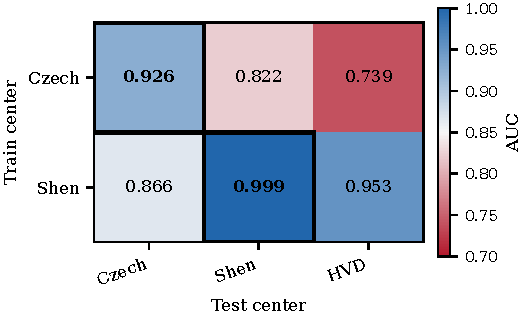
\includegraphics[width=\columnwidth]{Fig1.pdf}
\caption{AUC for ROP presence with a DINOv2 linear probe. Rows are training
centers and columns are test sets. Shen denotes Shenzhen, and HVD denotes
HVDROPDB, which lacks patient identifiers and is used only as an external test set}
\label{fig:crosssite}
\end{figure}

\begin{table*}[t]\centering\footnotesize
\caption{AUC (95\% bootstrap CI) for ROP presence with a DINOv2 linear probe.
Parentheses mark within-center testing. Shen denotes Shenzhen, and HVD denotes
HVDROPDB external testing. Bootstrap resampling used patient clusters when
available and image clusters for HVDROPDB}
\label{tab:crosssite}
\begin{tabular*}{0.82\textwidth}{@{\extracolsep{\fill}}llll@{}}
\toprule
train$\backslash$test & Czech & Shen & HVD \\ \midrule
Czech    & (0.926 [.826--.981]) & 0.822 [.789--.854] & 0.739 [.664--.810] \\
Shenzhen & 0.866 [.755--.921] & (0.999 [.996--1.000]) & 0.953 [.925--.978] \\
\bottomrule
\end{tabular*}
\end{table*}

\begin{figure*}[tbp]\centering
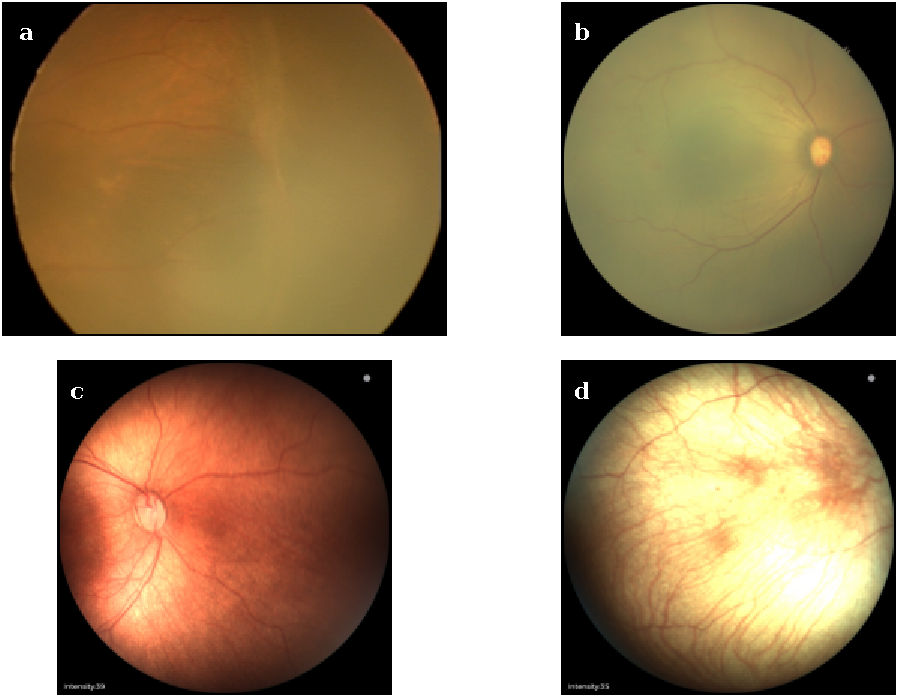
\includegraphics[width=0.84\textwidth]{Fig2.pdf}
\caption{Representative high-confidence source-to-target failure examples. Images
are de-identified public fundus photographs selected only for visualization after
model fitting. (a) False-negative HVDROPDB ROP image under Czech training,
\(p_{\mathrm{ROP}}<0.01\). (b) False-positive HVDROPDB normal image under Czech
training, \(p_{\mathrm{ROP}}>0.99\). (c) False-negative Czech active ROP image
under Shenzhen training, \(p_{\mathrm{ROP}}<0.01\). (d) False-positive Czech
no-active-ROP image under Shenzhen training, \(p_{\mathrm{ROP}}>0.99\)}
\label{fig:failures}
\end{figure*}

\subsection{Frozen representation results under matched probe settings}\label{sec:r-spectrum}
The backbone analysis was exploratory and implementation-specific. Under matched
$224{\times}224$ frozen linear-probe settings, the results did not follow a
simple specialist-over-generalist ordering. Across the cross-center and HVDROPDB
external-test rows, DINOv2, CLIP and ImageNet reached mean AUCs of 0.862, 0.844
and 0.838, respectively, compared with 0.761 for RETFound
(Table~\ref{tab:spectrum}). Under paired bootstrap testing, DINOv2 exceeded
RETFound significantly in three rows and was not significantly worse in any row
(Table~\ref{tab:bootstrap}; Fig.~\ref{fig:forest}). These results support only
the narrower statement that, under this frozen-probe implementation, RETFound did
not outperform the general-purpose backbones.

\begin{figure}[tbp]\centering
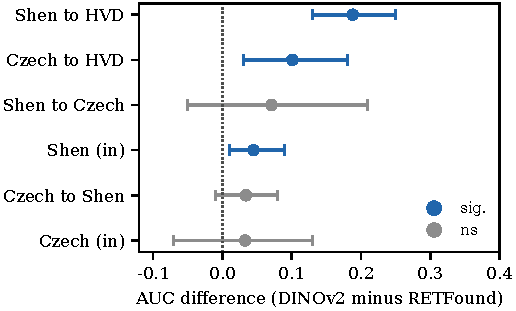
\includegraphics[width=\columnwidth]{Fig3.pdf}
\caption{Paired DINOv2 and RETFound comparison on ROP presence. Values are
paired AUC differences from the same test predictions.
Intervals come from a paired bootstrap with patient clusters when available and
image clusters for HVD. Shen denotes Shenzhen, and HVD denotes HVDROPDB. Blue
intervals exclude zero}
\label{fig:forest}
\end{figure}

The same ordering was observed in the 100\% data fine-tuning experiment trained on
Czech and evaluated on Czech, Shenzhen and HVDROPDB. DINOv2 reached AUCs of 0.90,
0.93 and 0.86; RETFound reached 0.77, 0.84 and 0.78; and random initialization
reached 0.52, 0.70 and 0.61. This single-source fine-tuning check was not
designed to establish a general ranking across retinal foundation models.

\begin{table}[t]\centering\scriptsize
\caption{Backbone spectrum for ROP presence using frozen linear probes at 224
pixel input resolution. Cz denotes Czech, Shen denotes Shenzhen, HVD denotes
HVDROPDB and RETF denotes RETFound. The transfer mean is computed over the
cross-center and HVD external-test rows}
\label{tab:spectrum}
\setlength{\tabcolsep}{2.5pt}
\begin{tabular*}{\columnwidth}{@{\extracolsep{\fill}}lcccc@{}}
\toprule
direction & DINOv2 & CLIP & ImageNet & RETF \\
 & SSL & V-L & sup. & retinal \\ \midrule
Czech (in)       & 0.893 & 0.845 & 0.866 & 0.854 \\
Shen (in)        & 0.991 & 0.992 & 0.988 & 0.947 \\
Cz$\to$Shen      & 0.851 & 0.827 & 0.845 & 0.816 \\
Shen$\to$Cz      & 0.786 & 0.803 & 0.828 & 0.707 \\
Cz$\to$HVD       & 0.861 & 0.845 & 0.760 & 0.760 \\
Shen$\to$HVD     & 0.948 & 0.902 & 0.920 & 0.760 \\ \midrule
\textbf{mean} & \textbf{0.862} & \textbf{0.844} & \textbf{0.838} & \textbf{0.761} \\
\bottomrule
\end{tabular*}
\end{table}

\begin{table}[t]\centering\scriptsize
\caption{Paired DINOv2 versus RETFound comparison for ROP presence with frozen
probes at 224 pixel input resolution. Shen denotes Shenzhen, and HVD denotes
HVDROPDB external testing. The paired bootstrap uses 2{,}000 resamples}
\label{tab:bootstrap}
\setlength{\tabcolsep}{2pt}
\begin{tabular*}{\columnwidth}{@{\extracolsep{\fill}}lrrcc@{}}
\toprule
direction & DINOv2 & RETF & $\Delta$ [95\% CI] & sig. \\ \midrule
Shen (in)        & 0.991 & 0.947 & $+0.045$ [.01, .09] & \checkmark \\
Cz$\to$HVD       & 0.861 & 0.760 & $+0.101$ [.03, .18] & \checkmark \\
Shen$\to$HVD     & 0.947 & 0.760 & $+0.188$ [.13, .25] & \checkmark \\
Czech (in)       & 0.886 & 0.854 & $+0.033$ [$-$.07, .13] & ns \\
Cz$\to$Shen      & 0.850 & 0.816 & $+0.034$ [$-$.01, .08] & ns \\
Shen$\to$Cz      & 0.778 & 0.707 & $+0.071$ [$-$.05, .21] & ns \\
\bottomrule
\end{tabular*}
\end{table}

\subsection{Sparse grader labels changed evaluable subsets and apparent performance}\label{sec:r-annot}
FARFUM-RoP contains sparse grader-specific plus disease labels from five graders,
not complete five-grader labels for every image. A single DINOv2 model trained on
consensus-style labels was evaluated separately against each grader's available
labels. Across these grader-specific evaluable subsets, AUC ranged from 0.930 to
0.996 (\(\Delta=0.066\)). Human-human Cohen $\kappa$, computed only on overlapping
labels, had mean 0.806 and ranged from 0.671 to 1.000. Model-grader agreement had
mean 0.784 and ranged from 0.494 to 0.908 (Fig.~\ref{fig:kappa}). This AUC spread
should not be interpreted as a pure grader-reference effect because the evaluable
image subset also changed across graders. It shows that sparse grader labels can
alter both the reference label and the test subset used to estimate model
performance.

\begin{figure}[tbp]\centering
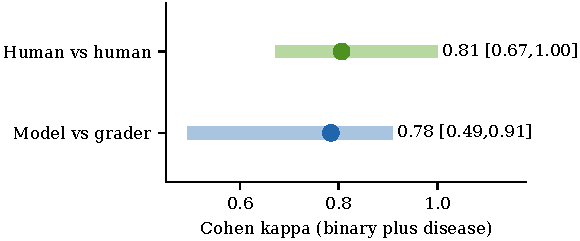
\includegraphics[width=\columnwidth]{Fig4.pdf}
\caption{Agreement on FARFUM-RoP plus disease using sparse multi-rater labels.
Human-human agreement is computed only on overlapping grader labels. Model-grader
agreement overlaps part of the inter-grader range but has a lower minimum value,
so single-annotator labels should be treated as uncertain}
\label{fig:kappa}
\end{figure}

\section{Discussion}\label{sec:discussion}
This study shows that performance estimates from public ROP datasets changed
with the source dataset and the available label reference. Within-center AUCs
were higher than cross-center AUCs, and HVDROPDB external-test performance varied
by training source. The Shenzhen within-center result was nearly perfect, but
that result is also compatible with a curated or highly separable public dataset.
These findings are consistent with prior external validation work showing that
ROP AI models must be evaluated in the target imaging setting rather than assumed
to transfer from development data~\cite{coyner2022,coyner2024}.

The representation comparison should be interpreted within its implementation
limits. Under matched frozen-probe settings, RETFound did not outperform DINOv2,
CLIP or ImageNet features in this analysis, and the Czech fine-tuning check
showed the same ordering. This comparison does not isolate pretraining domain
from architecture, preprocessing, input resolution, linear-probe regularization or
fine-tuning seed. It supports the practical conclusion that model rankings in
public ROP datasets should be checked under the intended evaluation protocol.

The FARFUM-RoP annotator analysis highlights a separate limitation of public
labels. The grader-specific AUC spread combines differences in reference labels
with differences in the evaluable image subsets, because the five graders did not
label the same complete image set. Plus disease is also known to have imperfect
expert agreement~\cite{chiang2007}. ROP AI studies should report whether labels
come from consensus, single-grader or sparse multi-grader annotations, and should
avoid treating one available grader label as a perfect reference standard.

Public ROP datasets make independent comparison possible, but they were not
collected with a shared protocol. This study quantifies performance loss across
source changes and label-reference changes that would be missed by pooled or
single-source evaluation. Future validation studies should prespecify
patient-level splits, report camera or acquisition strata, include image-quality
assessment and use multi-rater adjudication where feasible.

\subsection{Limitations}\label{sec:limitations}
ROP-positive patients are scarce in public data, which limits subgroup slicing.
The primary endpoint was active ROP presence rather than referable ROP or
treatment requiring ROP. This endpoint was chosen because referable ROP and plus
disease labels were not available with enough positive patients for cross-center
transfer analysis across public datasets. The plus-disease task is secondary and
patient-limited. We did not have enough positive cases for
a population controlled device analysis within one center, so this benchmark
should not be read as a validation study stratified by device. Shenzhen is curated
and nearly separable in distribution. HVDROPDB is small, with 185 images and no
patient identifiers, so it is used only as an external test set in the primary
analysis. Labels are mostly consensus single annotations, and FARFUM-RoP's
multi-rater labels are sparse rather than complete five-grader labels. We did not
perform a matched-overlap grader analysis because the overlap among non-abstention
grader labels was limited. We did not perform external prospective clinical
validation.

\backmatter

\bmhead{Acknowledgements}
None.

\bmhead{Declarations}

\textbf{Funding} No funding was received for this work.

\textbf{Competing interests} The authors declare no competing interests.

\textbf{ORCID} Jin Luo: \url{https://orcid.org/0009-0007-1277-7692}.

\textbf{Author contact information} Jin Luo: \url{luojin@xmu.edu.cn}; Dongwei
Guo: \url{guodongwei1518@foxmail.com}; Xinsi Chen:
\url{chenxinsi1016@163.com}; Hao Liang: \url{hl106@rice.edu}; Fang Lin:
\url{cesare_l@icloud.com}.

\textbf{Ethics approval and consent to participate} This study is a secondary
analysis of publicly available de-identified datasets. No new human participant
data were collected, and no additional institutional ethics approval was required
for this analysis.

\textbf{Consent for publication} Not applicable. No identifiable individual
participant information is reported.

\textbf{Data availability} The datasets analyzed in this study are publicly
available from the sources cited in the manuscript. The harmonization manifest,
split files and analysis artifacts generated for this study are archived on
Zenodo at \url{https://doi.org/10.5281/zenodo.20721027}.

\textbf{Materials availability} Not applicable.

\textbf{Code availability} The analysis code is available at
\url{https://github.com/foye80/rop-bench} and archived on Zenodo at
\url{https://doi.org/10.5281/zenodo.20721027}.

\textbf{Author contributions} Jin Luo conceived the study, performed the
analyses, interpreted the results and drafted the manuscript. Dongwei Guo, Xinsi
Chen and Fang Lin contributed clinical interpretation and manuscript revision.
Hao Liang contributed data analysis support, code review and manuscript revision.
All authors reviewed and approved the final manuscript.

\textbf{Use of artificial intelligence tools} Artificial intelligence tools were
used for language editing and manuscript formatting under author supervision. The
authors reviewed the final manuscript and take responsibility for all content.

\begin{thebibliography}{99}

\bibitem{blencowe2013}
Blencowe H, Lawn JE, Vazquez T, Fielder A, Gilbert C (2013)
Preterm-associated visual impairment and estimates of retinopathy of prematurity
at regional and global levels for 2010. Pediatr Res 74:35-49.
\url{https://doi.org/10.1038/pr.2013.205}

\bibitem{coyner2022}
Coyner AS, Oh MA, Shah PK, Singh P, Ostmo S, Valikodath NG, et al (2022)
External validation of a retinopathy of prematurity screening model using
artificial intelligence in 3 low- and middle-income populations. JAMA Ophthalmol
140:791-798. \url{https://doi.org/10.1001/jamaophthalmol.2022.2135}

\bibitem{icrop3}
Chiang MF, Quinn GE, Fielder AR, Ostmo SR, Chan RVP, Berrocal A, et al (2021)
International Classification of Retinopathy of Prematurity, Third Edition.
Ophthalmology 128:e51-e68. \url{https://doi.org/10.1016/j.ophtha.2021.05.031}

\bibitem{brown2018}
Brown JM, Campbell JP, Beers A, Chang K, Ostmo S, Chan RVP, et al (2018)
Automated diagnosis of plus disease in retinopathy of prematurity using deep
convolutional neural networks. JAMA Ophthalmol 136:803-810.
\url{https://doi.org/10.1001/jamaophthalmol.2018.1934}

\bibitem{campbell2021ai}
Campbell JP, Singh P, Redd TK, Brown JM, Shah PK, Subramanian P, et al (2021)
Applications of artificial intelligence for retinopathy of prematurity screening.
Pediatrics 147:e2020016618. \url{https://doi.org/10.1542/peds.2020-016618}

\bibitem{coyner2024}
Coyner AS, Murickan T, Oh MA, Young BK, Ostmo SR, Singh P, et al (2024)
Multinational external validation of autonomous retinopathy of prematurity
screening. JAMA Ophthalmol 142:327-335.
\url{https://doi.org/10.1001/jamaophthalmol.2024.0045}

\bibitem{retfound2023}
Zhou Y, Chia MA, Wagner SK, Ayhan MS, Williamson DJ, Struyven RR, et al (2023)
A foundation model for generalizable disease detection from retinal images.
Nature 622:156-163. \url{https://doi.org/10.1038/s41586-023-06555-x}

\bibitem{chiang2007}
Chiang MF, Jiang L, Gelman R, Du YE, Flynn JT (2007) Interexpert agreement of
plus disease diagnosis in retinopathy of prematurity. Arch Ophthalmol
125:875-880. \url{https://doi.org/10.1001/archopht.125.7.875}

\bibitem{farfum2024}
Akbari M, Pourreza HR, Khalili Pour E, Dastjani Farahani A, Bazvand F,
Ebrahimiadib N, et al (2024) FARFUM-RoP: a dataset for computer-aided detection
of retinopathy of prematurity. Sci Data 11:1176.
\url{https://doi.org/10.1038/s41597-024-03897-7}

\bibitem{shenzhen2024}
Zhao X, Chen S, Zhang S, Liu Y, Hu Y, Yuan D, et al (2024) A fundus image
dataset for intelligent retinopathy of prematurity system. Sci Data 11:543.
\url{https://doi.org/10.1038/s41597-024-03362-5}

\bibitem{hvdropdb2023}
Agrawal R, Walambe R, Kotecha K, Gaikwad A, Deshpande M, Kulkarni S (2024)
HVDROPDB datasets for research in retinopathy of prematurity. Data Brief
52:109839. \url{https://doi.org/10.1016/j.dib.2023.109839}

\bibitem{czech2024}
Timkovi{\v{c}} J, Nov{\'a}kov{\'a} J, Kub{\'i}{\v{c}}ek J, Hasal M,
Vary{\v{s}}ov{\'a} A, Kolar{\v{c}}{\'i}k L, et al (2024) Retinal image dataset of
infants and retinopathy of prematurity. Sci Data 11:814.
\url{https://doi.org/10.1038/s41597-024-03409-7}

\bibitem{dinov2}
Oquab M, Darcet T, Moutakanni T, Vo H, Szafraniec M, Khalidov V, et al (2024)
DINOv2: learning robust visual features without supervision. Trans Mach Learn
Res. arXiv:2304.07193

\bibitem{clip2021}
Radford A, Kim JW, Hallacy C, Ramesh A, Goh G, Agarwal S, et al (2021)
Learning transferable visual models from natural language supervision. In:
Proceedings of the 38th International Conference on Machine Learning. PMLR
139:8748-8763.

\end{thebibliography}
\end{document}
